%%% Laboratory	 Notes
%%% Template by Mikhail Klassen, April 2013
%%% Contributions from Sarah Mount, May 2014
\documentclass[a4paper]{tufte-handout}

\newcommand{\workingDate}{\textsc{Mar. $|$ 2023}}
\newcommand{\userName}{\AE ther Zhou}
% \newcommand{\institution}{Your University}

\usepackage{lab_notes}
\usepackage{siunitx}

\usepackage{hyperref}
\hypersetup{
    pdffitwindow=false,            % window fit to page
    pdfstartview={Fit},            % fits width of page to window
    pdftitle={Lab notes 2014},     % document title
    pdfauthor={Your Name},         % author name
    pdfsubject={},                 % document topic(s)
    pdfnewwindow=true,             % links in new window
    colorlinks=true,               % coloured links, not boxed
    linkcolor=DarkScarletRed,      % colour of internal links
    citecolor=DarkChameleon,       % colour of links to bibliography
    filecolor=DarkPlum,            % colour of file links
    urlcolor=DarkSkyBlue           % colour of external links
}


\title{PHYS 128AL Lab Notebook}
\author[]{\AE ther Zhou}
\date{Feb. 2023}

\begin{document}
\maketitle
%%%%%%%%%%%%%%%%%%%%%%%%%%%%%%%%%%%%%%%%%%%%%%%%%%%%%%%%

\begin{projects}
	\begin{description}
        \item [Lab 3] Noise 
		\item [Collaborator] Vivian Liao
		\end{description}
\end{projects}

%%%%%%%%%%%%%%%%%%%%%%%%%%%%%%%%%%%%%%%%%%%%%%%%%%%%%%%%
\tableofcontents

\newpage

%%%%%%%%%%%%%%%%%%%%%%%%%%%%%%%%%%%%%%%%%%%%%%%%%%%%%%%%
\section{Lab Manuel Questions}

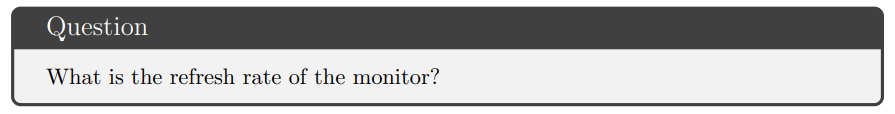
\includegraphics[width = 1\textwidth]{figures/q1.png}

60 Hz 

\hrulefill

%%%%%%%%%%%%%%%%%%%%%%%%%%%%%%%%%%%%%%%%%%%%%%%%%%%%%%%%
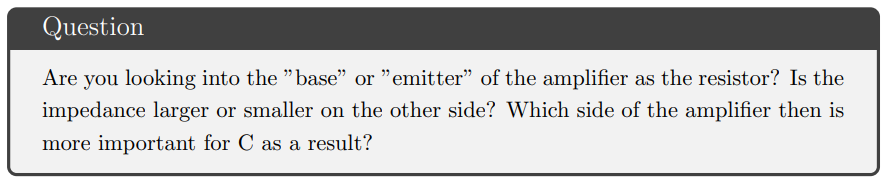
\includegraphics[width = 1\textwidth]{figures/q2.png}

emitter (higher voltage require higher impedance)

\hrulefill

%%%%%%%%%%%%%%%%%%%%%%%%%%%%%%%%%%%%%%%%%%%%%%%%%%%%%%%%
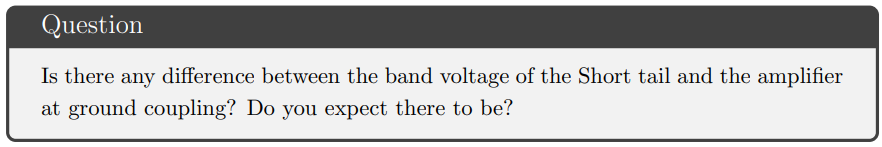
\includegraphics[width = 1\textwidth]{figures/q3.png}

No difference. When we shorted the analyzer, we are equalizing the electric potential on both polar, which is the same as amplifier at ground coupling.

% #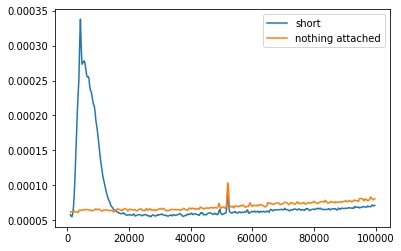
\includegraphics[width = 1\textwidth]{figures/q3a.png}

\hrulefill

%%%%%%%%%%%%%%%%%%%%%%%%%%%%%%%%%%%%%%%%%%%%%%%%%%%%%%%%
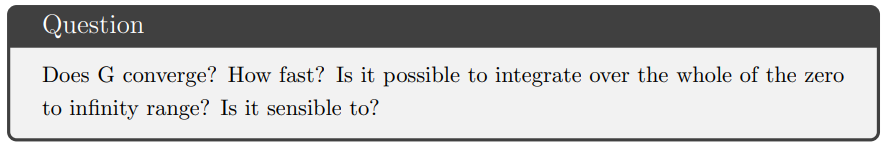
\includegraphics[width = 1\textwidth]{figures/q4.png}

The band gain has a Gaussian-like distribution, it should converge as fast as a Gaussian distribution. Hence, it is possible to integrate over the whole domain. However, we don't need to, since the band gain almost dies out around 1-$\sigma$. It is more efficient to just integrate within a certain bandwidth.

\hrulefill

%%%%%%%%%%%%%%%%%%%%%%%%%%%%%%%%%%%%%%%%%%%%%%%%%%%%%%%%
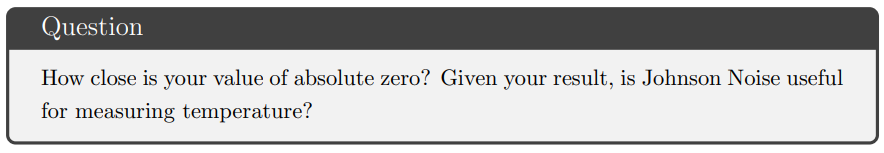
\includegraphics[width = 1\textwidth]{figures/q5.png}

Our final result suggests the absolute zero to be $-286\pm 16\,\si{^\circ C}$, which is within 5\% of the accepted value. So it is useful to measure temperature with Johnson Noise.

\hrulefill

%%%%%%%%%%%%%%%%%%%%%%%%%%%%%%%%%%%%%%%%%%%%%%%%%%%%%%%%
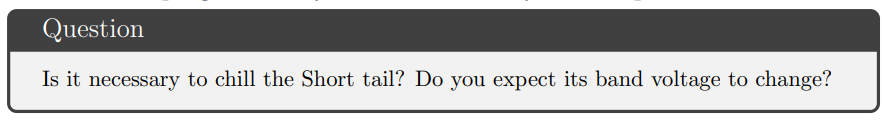
\includegraphics[width = 1\textwidth]{figures/q6.png}

For an ideally short wire, its resistance should be zero regardless of the temperature. So we expect the result to be the same.

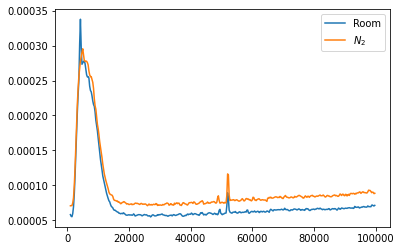
\includegraphics[width = 1\textwidth]{figures/q6a.png}

\hrulefill

%%%%%%%%%%%%%%%%%%%%%%%%%%%%%%%%%%%%%%%%%%%%%%%%%%%%%%%%
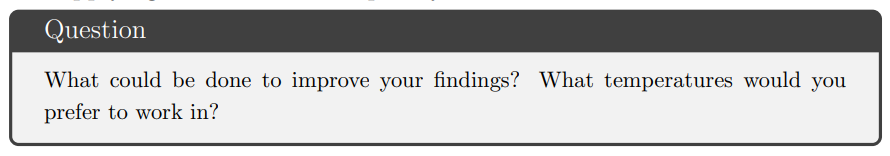
\includegraphics[width = 1\textwidth]{figures/q7.png}

Our measurement are affected by the background noise (Systematic error). We'll need to repeat more trails to figure out the noise generated by the analyzer itself, so we can measure the Johnson noise as accurate as possible.

It would be preferable to work with temperature slightly higher than the room temperature. So we can further verify Nyqiust's theorem on Johnson noise. 

\hrulefill

%%%%%%%%%%%%%%%%%%%%%%%%%%%%%%%%%%%%%%%%%%%%%%%%%%%%%%%%
\newpage

%%%%%%%%%%%%%%%%%%%%%%%%%%%%%%%%%%%%%%%%%%%%%%%%%%%%%%%%
\section{Daily}
\newday{22 Feb 2023, W}
\begin{itemize}
    \item {equipment set up: } {noise generator, pre-amplifier, filter, spectral analyzer}
    \item Room temperature measurement  ($20\pm 1$ Celsius)
    \item using floppy disk (bad reading, not saving data)
    
\end{itemize}
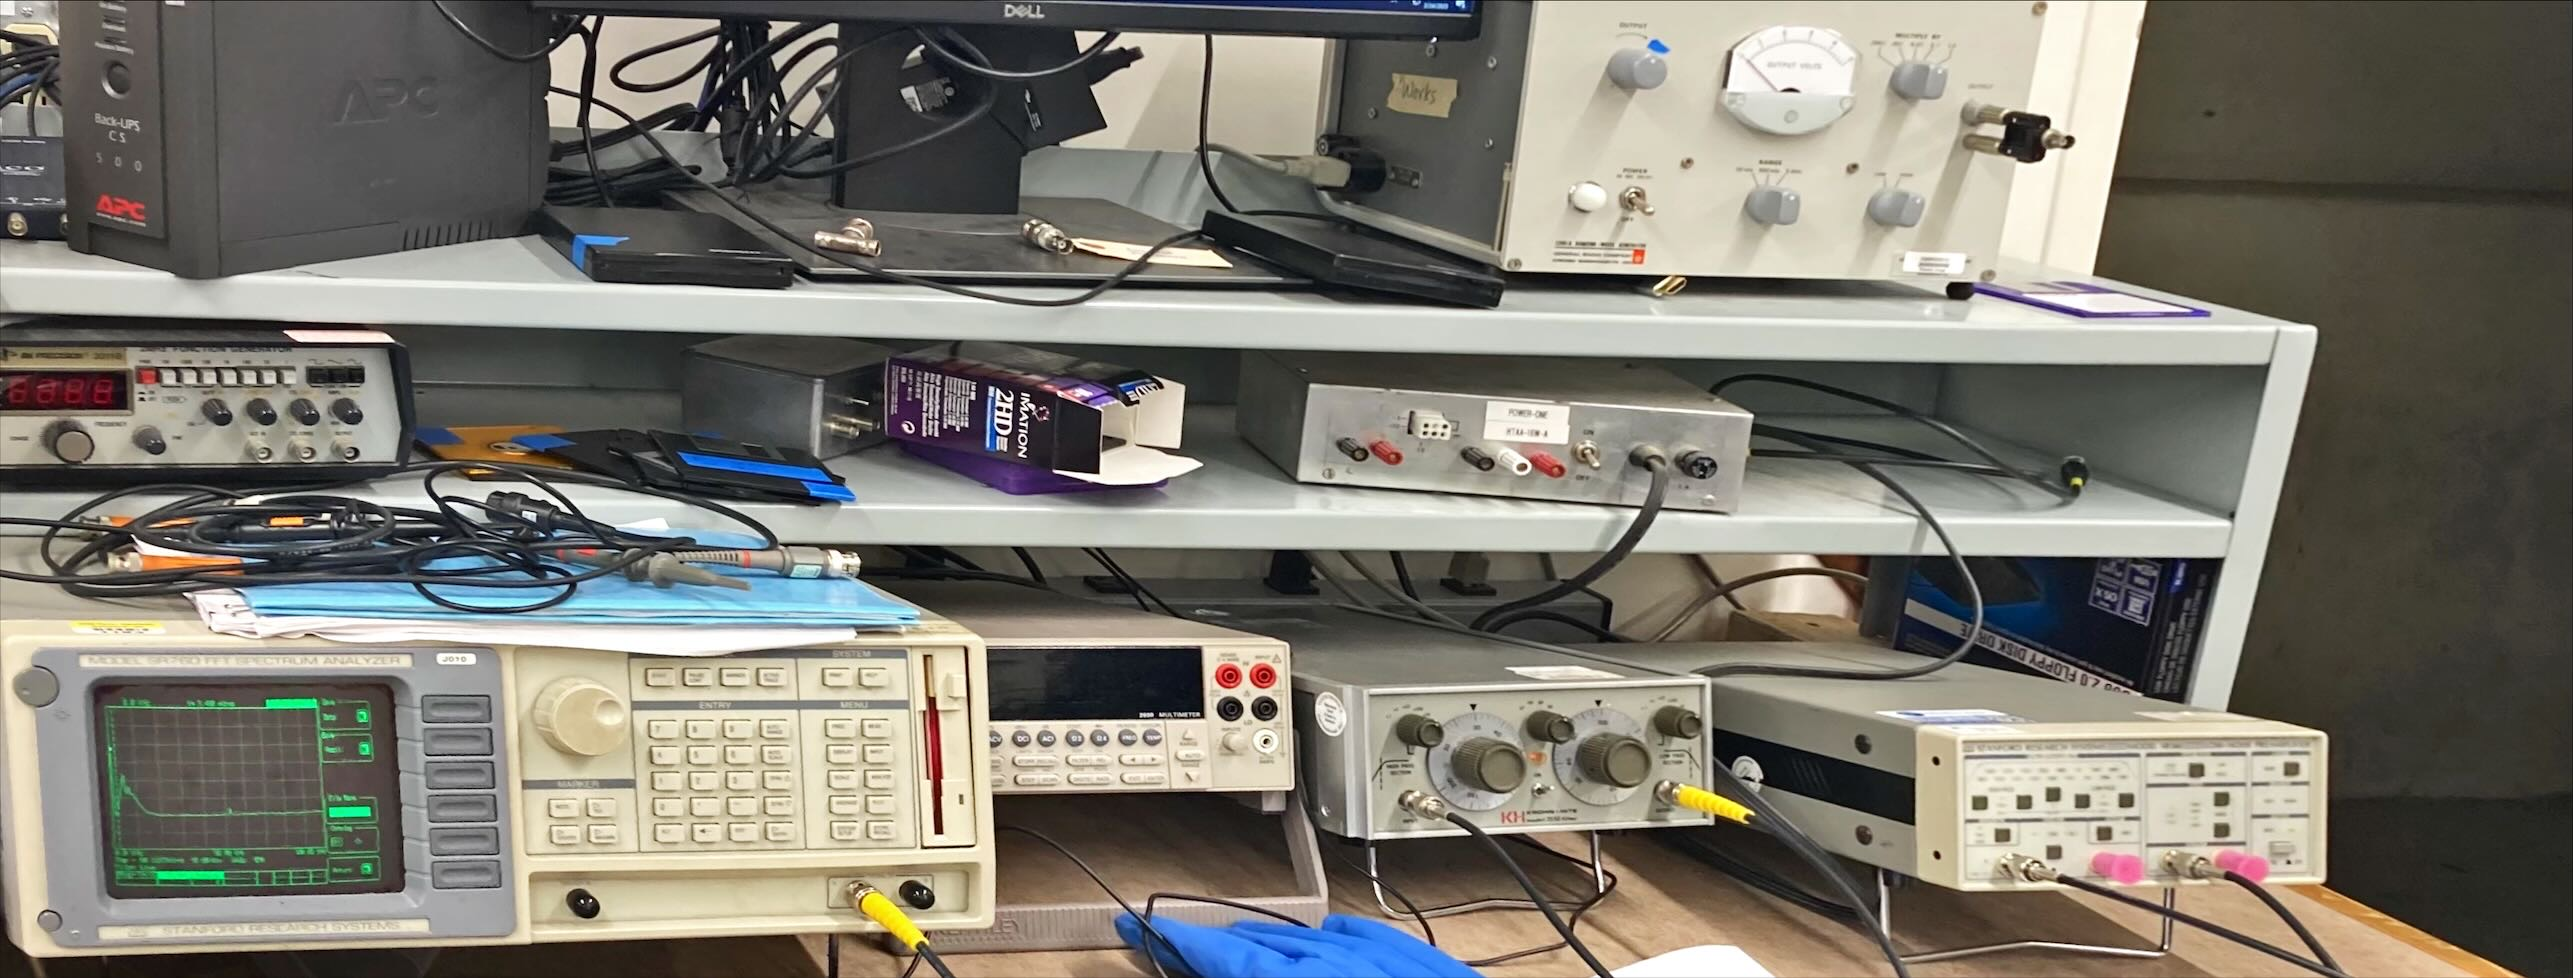
\includegraphics[width = 1 \textwidth]{figures/day1_setup.jpg}
\\

$$g(f) = \frac{V_{out}(f)}{V_{in}}$$
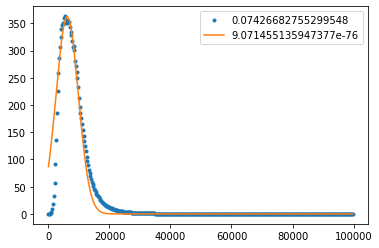
\includegraphics[width = 1 \textwidth]{figures/day1_gain.png}

\hrulefill

%%%%%%%%%%%%%%%%%%%%%%%%%%%%%%%%%%%%%%%%%%%%%%%%%%%%%%%%

\newday{24 Feb 2023, F}
\begin{itemize}
    \item measure resistor
    \item control temperature using boiling liquid nitrogen (77 Celsius)
    \item getting negative voltage reading (negative $V_{rms}$ doesn't make sense)
\end{itemize}

%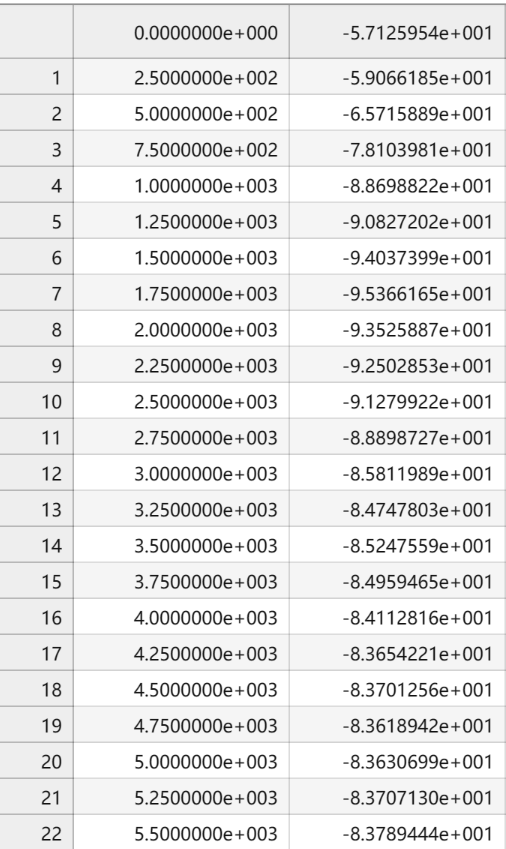
\includegraphics[width = 1     \textwidth]{figures/day2_bad1.png}

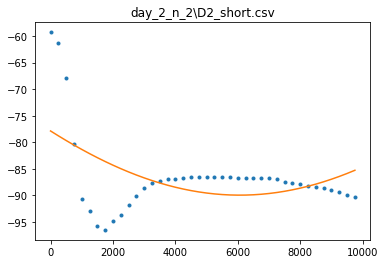
\includegraphics[width = 1     \textwidth]{figures/day2_bad.png}

Gain, band gain, temperature
$$G=\int_{0}^{\infty} \frac{[g(f)]^2}{1+(2\pi fCR)^2} \,df$$
Found capacitance C for coaxial cable to be 60 $pF/ft$
$$\text{slope} = T = \frac{V^2}{4k_BGR}$$
Using peak value for V (find max for each data set)

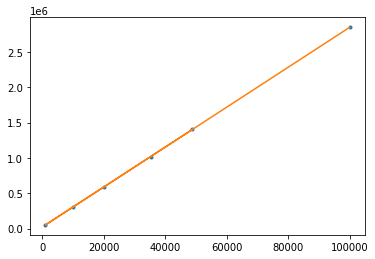
\includegraphics[width = 1 \textwidth]{figures/day2_room.png}

get 28 degree Kelvin, which is wrong

possible mistake: should use rms(V) not max(V)

\hrulefill

%%%%%%%%%%%%%%%%%%%%%%%%%%%%%%%%%%%%%%%%%%%%%%%%%%%%%%%%
\newday{27 Feb 2023, M}
Getting temperature offed by a factor of 4

measured capacitance (38 $pF/m$)

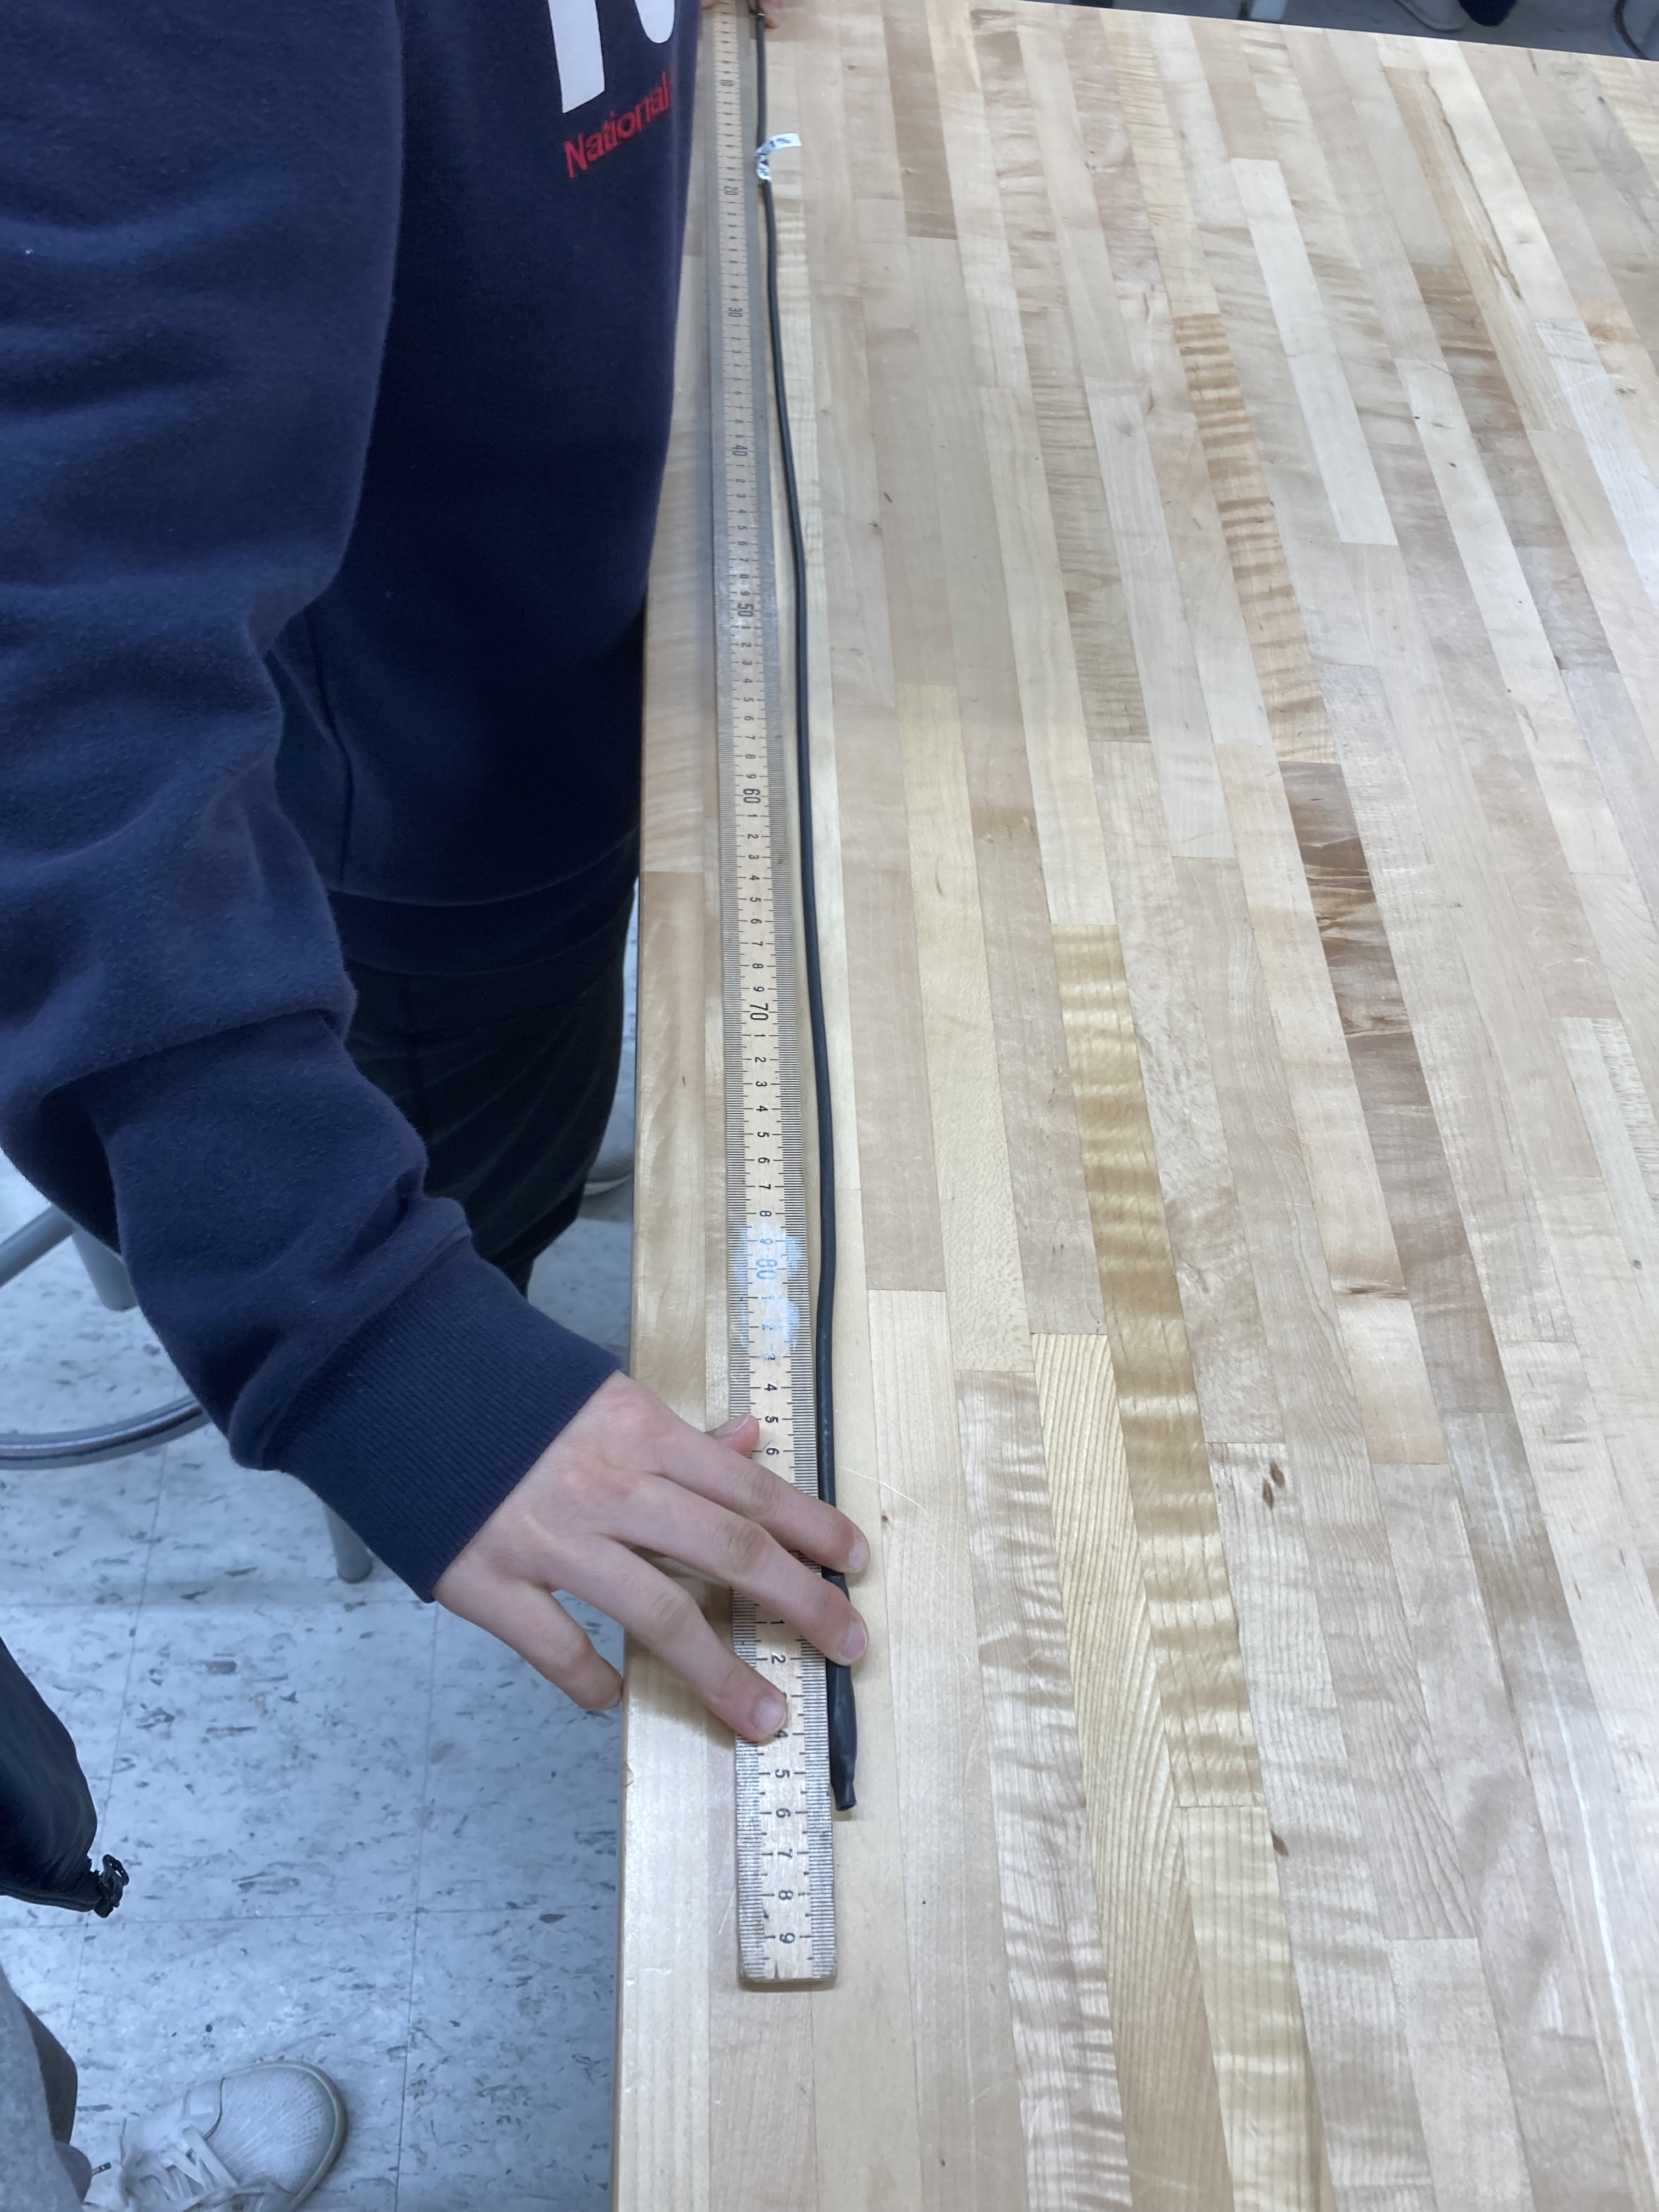
\includegraphics[angle=90,origin=c,width = 1 \textwidth]{figures/day3_cap.jpg}

With {scipy.curve\_fit()} Fitted data to get gain function (Gaussian fit)

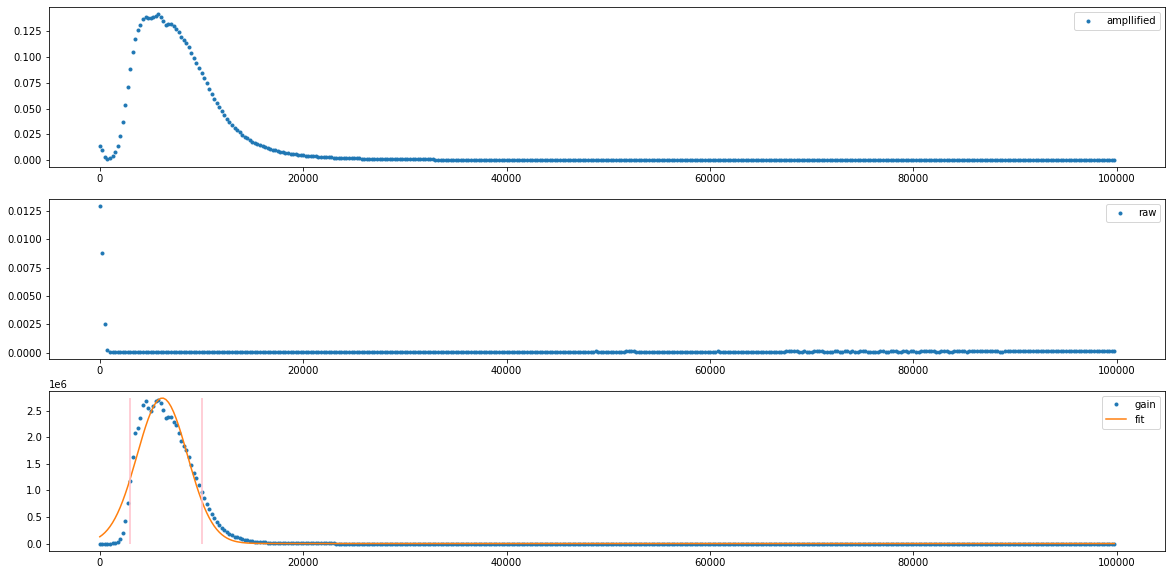
\includegraphics[width = 1.5\textwidth]{figures/day3_gain.png}

\hrulefill

%%%%%%%%%%%%%%%%%%%%%%%%%%%%%%%%%%%%%%%%%%%%%%%%%%%%%%%%
\newday{1 Mar 2023, W}
\begin{itemize}
    \item measured R to be check the 1\% error (checked)
    \item using band analyze function to get $V^2$
\end{itemize}
\begin{center}
    %\renewcommand{\arraystretch}{1.3}
    \centering
    \begin{tabular}{| l | c | c |}
    \hline
    R [k$\Omega$] & $V_{rms,~20^\circ C}$ [mV] & $V_{rms,~-195.79^\circ C}$ [mV]\\
    \hline
    \hline
    1 & 1.318 & 1.097\\
    10 & 3.281 & 2.065\\
    20 & 4.569 & 2.615\\
    35.2 & 5.878 & 3.329 \\
    48.7 & 6.804 & 3.895\\
    100 & 9.021 & 4.967\\
    short & 0.9291 & 0.9589 \\
    \hline
    $\frac{\delta R}{R} = 1\%$& $\frac{\delta V_{rms}}{V_{rms}} = 0.02\%$&$\frac{\delta V_{rms}}{V_{rms}} = 0.02\%$ \\
    \hline
    \end{tabular}

    
    \caption{Raw data of the band RMS voltage over the frequency band from 3 kHz to 10 kHz of different resistors under two different temperatures, $T=20~^\circ$C and $T=-195.79~^\circ$C.} \label{table:Vrms}
\end{center}

\begin{center}
    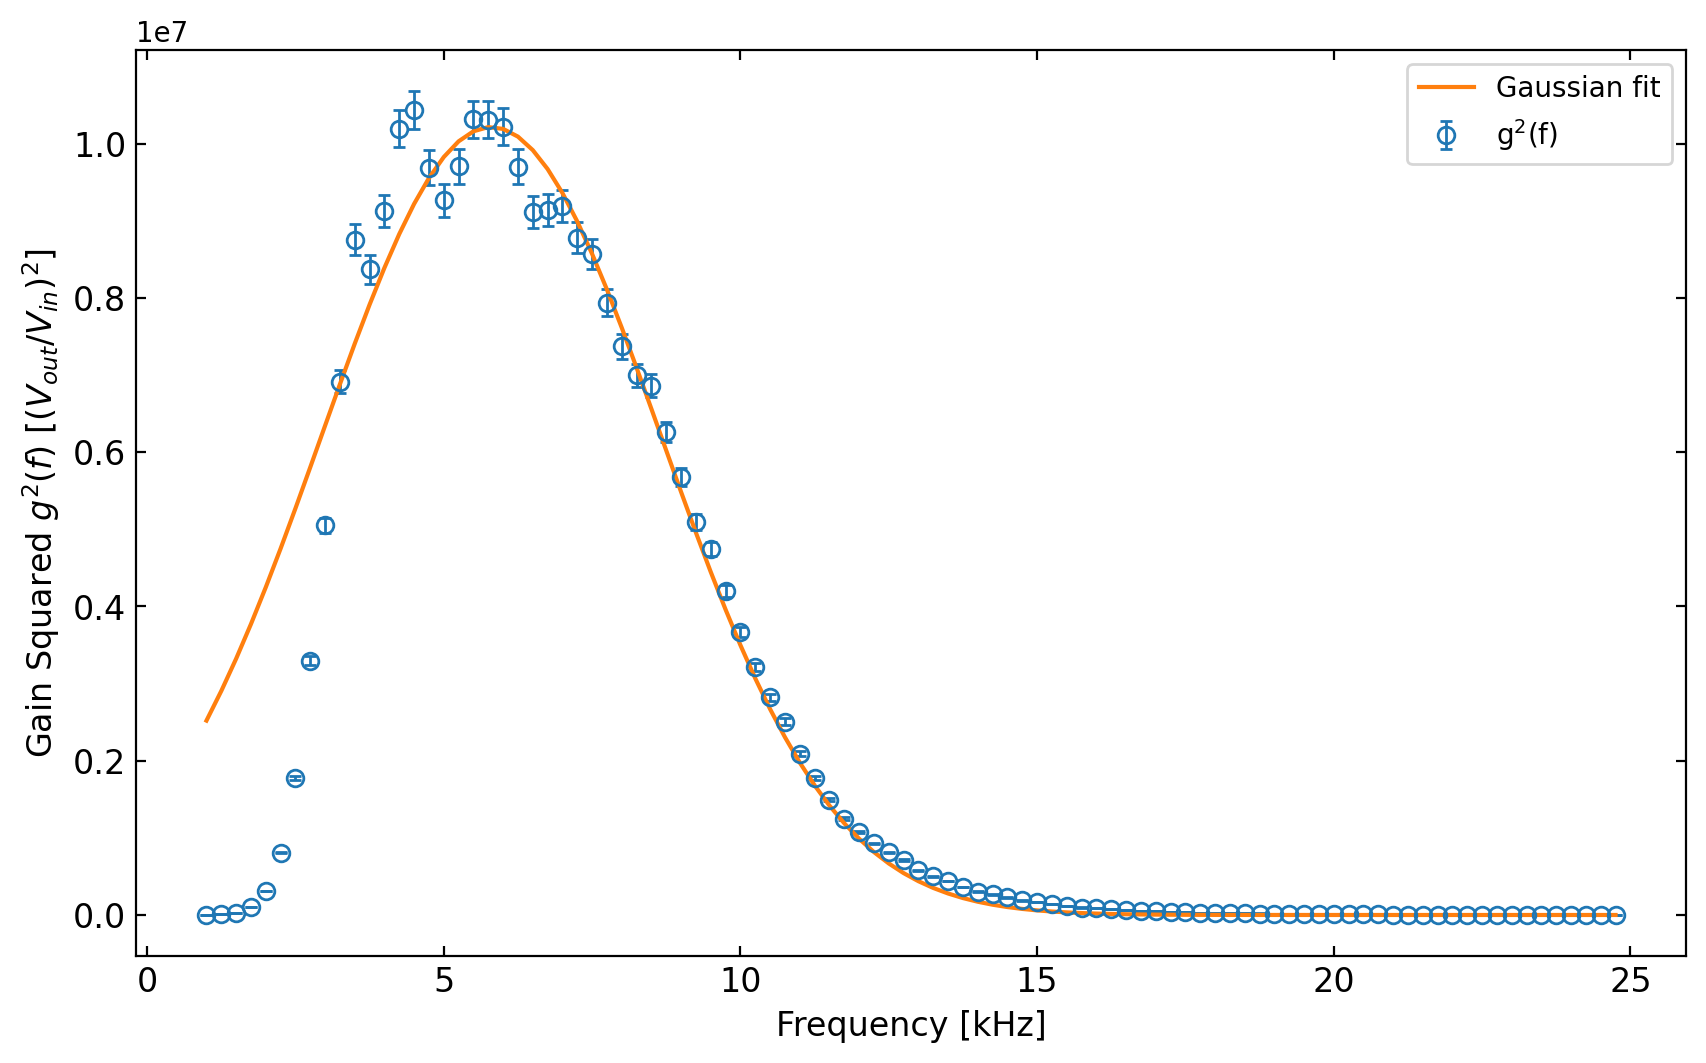
\includegraphics[width = 1\textwidth]{figures/day4_fit_gain.png}
    \caption{Fitted gain function using the signal from white noise generator. Since $g(f)$ is independent with the signal sources, We will use this to infer the actual magnitude of Johnson noise. We only care about the region between 3 kHz and 10 kHz.}\label{fig:gauss_fit}
\end{center}

\begin{center}
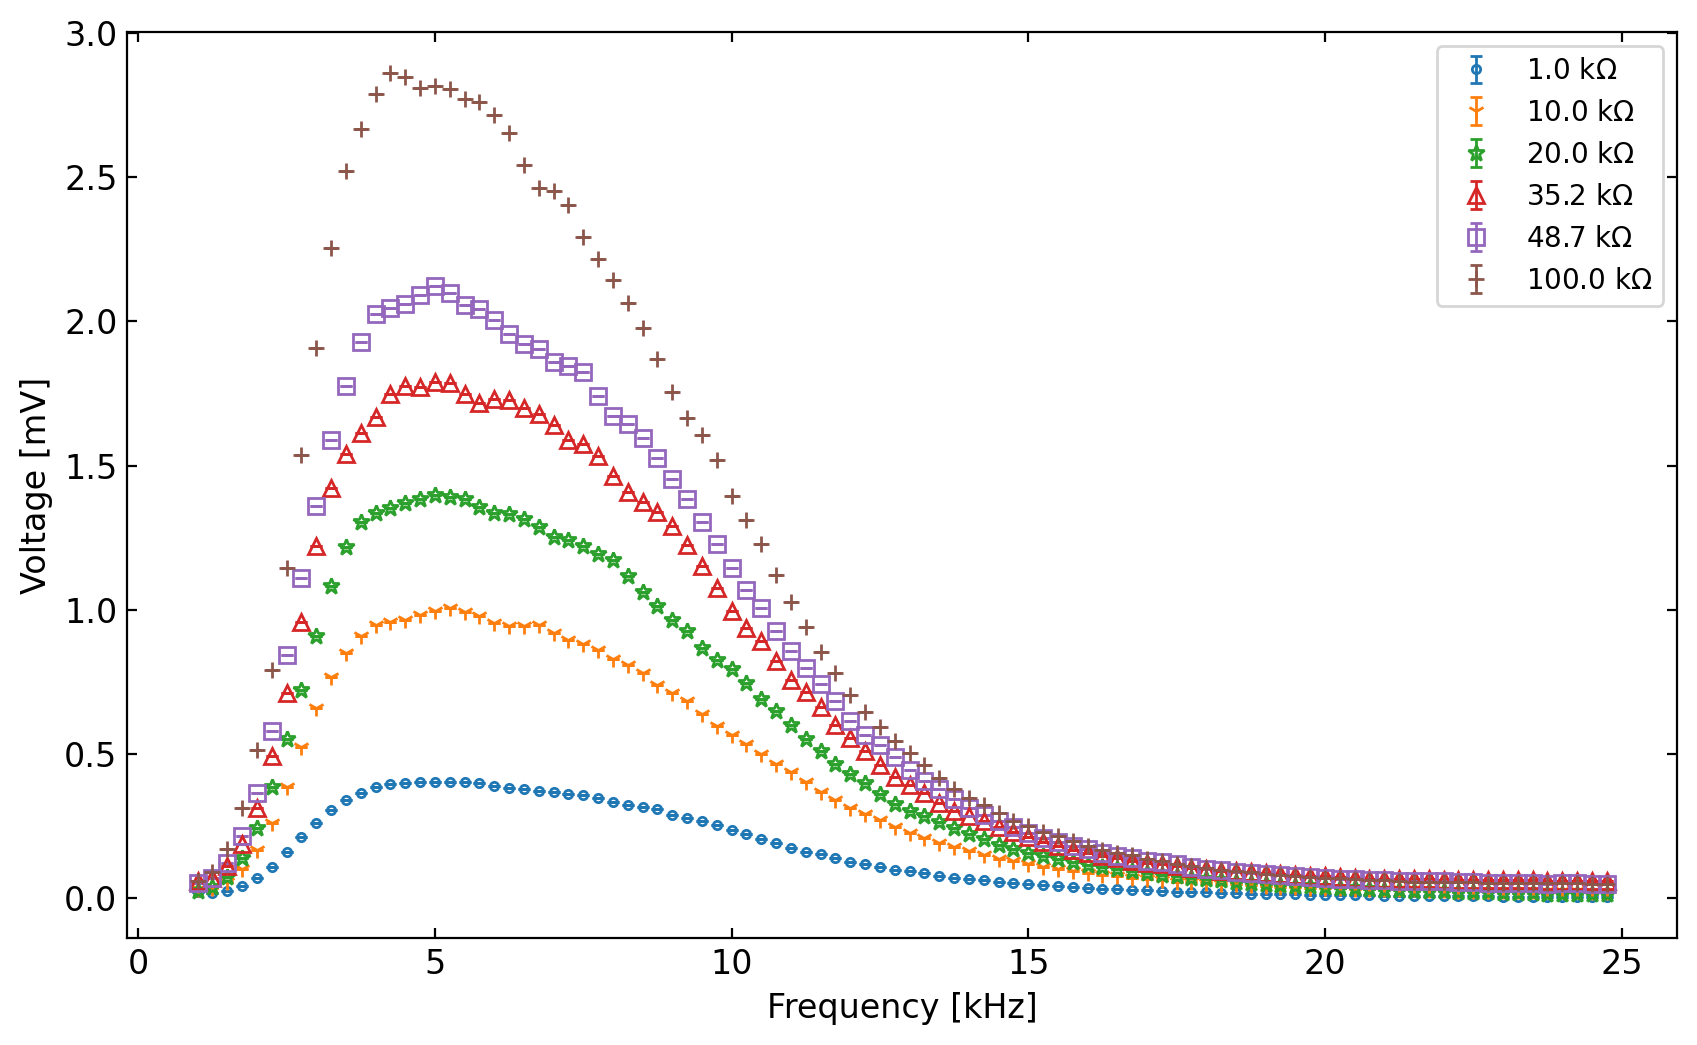
\includegraphics[width = 1\textwidth]{figures/day4_vres.png}
    \caption{Raw Data of the RMS voltage of different resistors under room temperature $T=20~^\circ$C. Different colored symbols represent the data point of different resistances. Error bars are presented.}
    \label{fig:raw data room temperature}
\end{center}



\newpage
\section{Theory and Setup}

\subsection{Set up and Procedure}

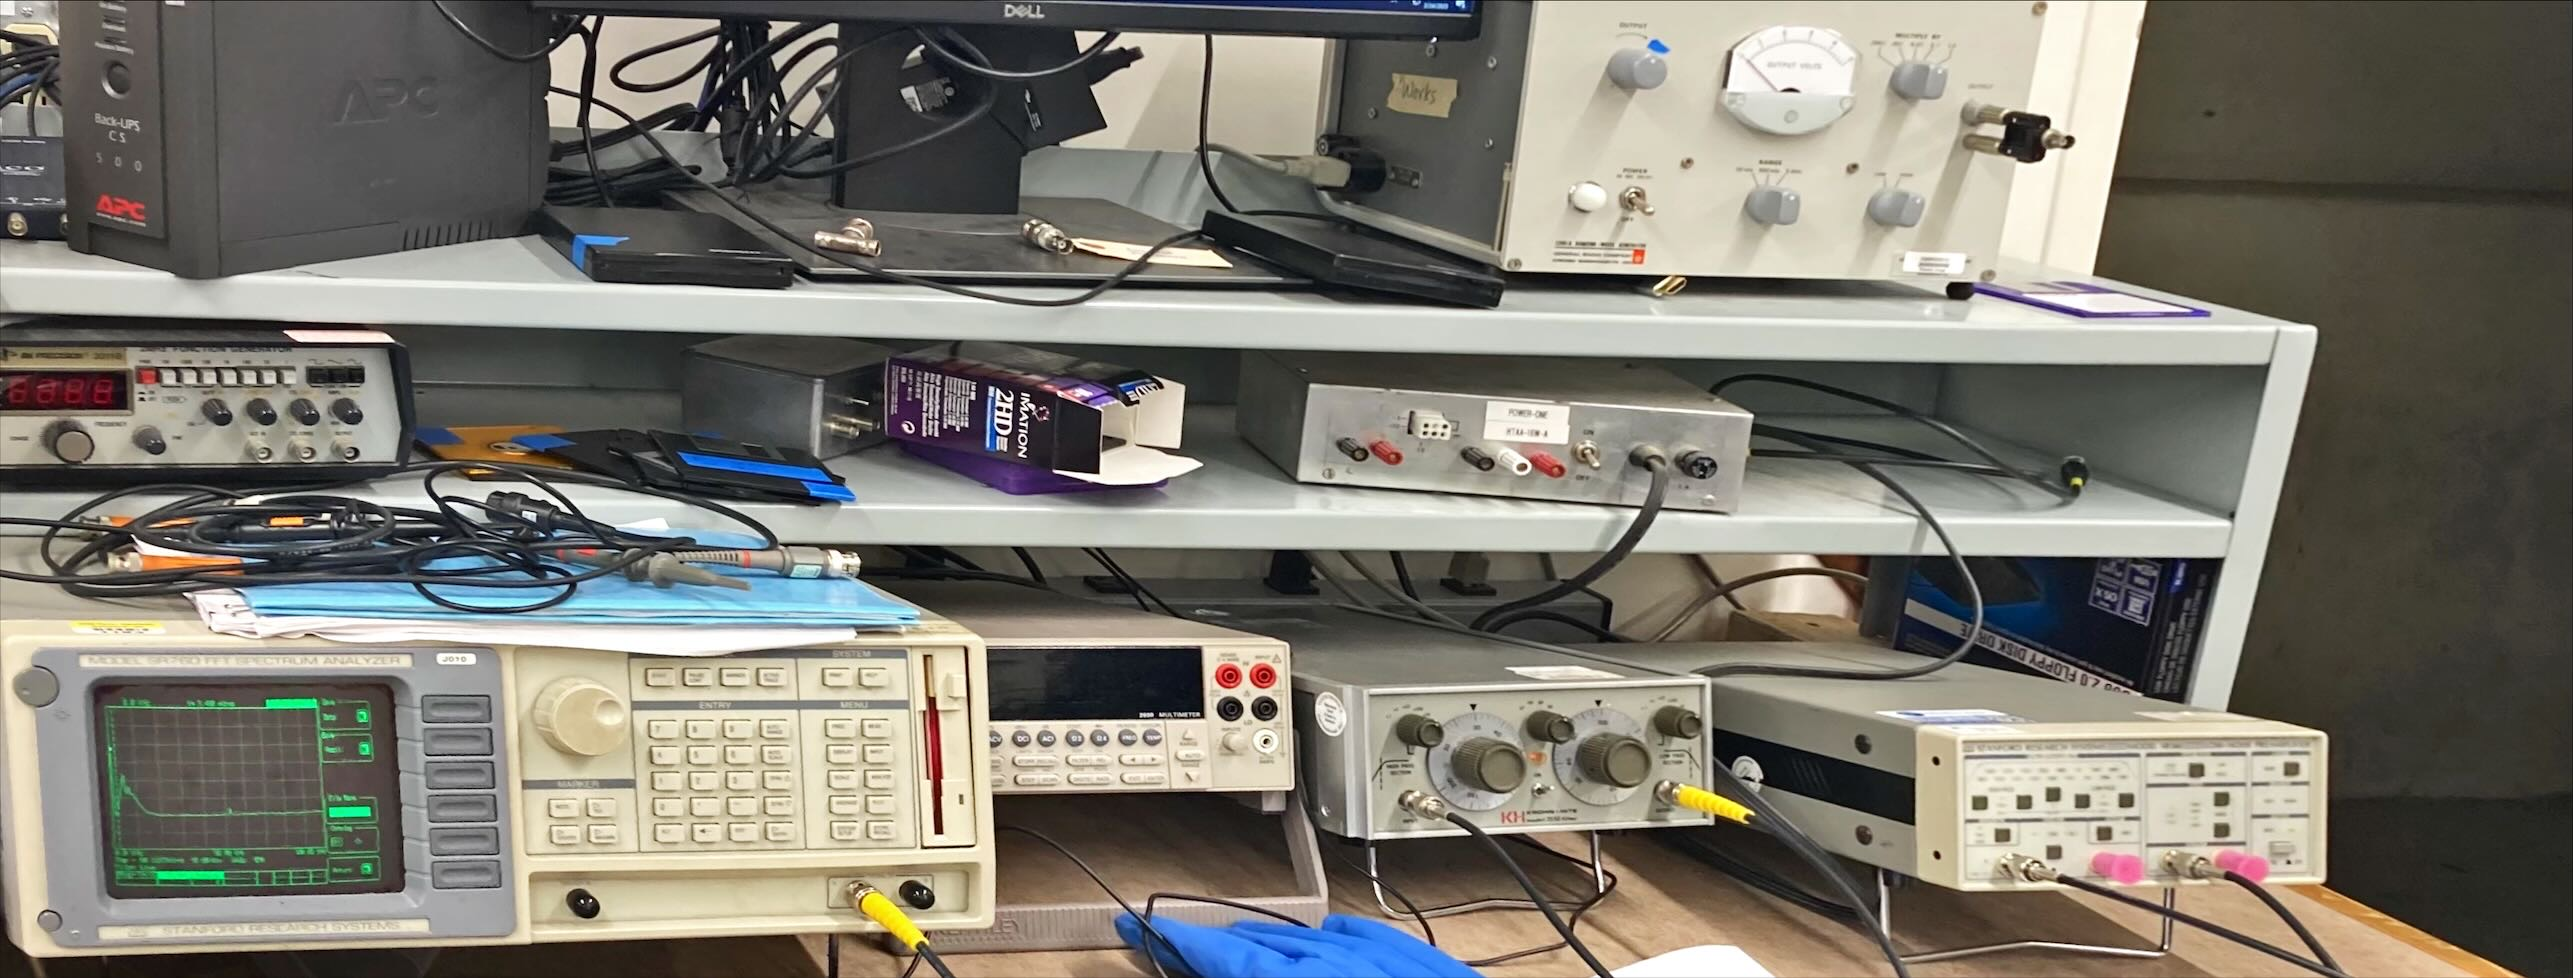
\includegraphics[width= 1 \linewidth]{figures/day1_setup.jpg}
Noise signal are pre-amplified, filtered to band of 3 kHz to 10 kHz, and fed into the spectral analyzer (FFT)

So we can see the physical property of Johnson noise. 

To calculate temperature or $k_B$, we need first restore our data to its original amplitude. So we need the gain function and the band gain.

$$g(f) = \frac{V_{out}(f)}{V_{in}}$$

$$G=\int_{0}^{\infty} \frac{[g(f)]^2}{1+(2\pi fCR)^2} \,df$$

By Nyquist
$$V^2=4k_BTGR$$
\quad Hence, by fixing $k_B$, we can give a measurement of temperature, and to derive the absolute zero in Celsius; and by fixing $T$ (using boiling liquid nitrogen), we can estimate the value of $k_B$.

The hard part is to calculate a clean band gain. Due to the high sensitivity, the spectral analyzer tends to take up lots of irrelevant background noise. 

In our experiment, we took several data for background noise of the analyzer itself (when nothing is attached to it). We tried analyze that to get a descriptive $V_b$, so we can minus it from the other signal data we took, and get the clean signal with background noise blocked. 

\newpage
\section{Result and Analysis}
\subsection{Experiment Result}
\quad By measuring the thermal noises of a series of shorted resistors with a filtered amplifier, we estimated absolute zero temperature to be $-286 \pm 16 \,\si{^\circ C}$, in agreement with the accepted value $-273.15\,\si{^\circ C}$. We also calculated the Boltzmann constant by controlling the temperature of the resistors. However, our calculated value $(1.665\pm 0.094)\times 10^{-23}\,\si{J\cdot K^{-1}}$ deviates from the accepted value $1.381\times 10^{-23}\,\si{J\cdot K^{-1}}$ by $21\%$. A possible cause for this discrepancy is the variation in background noise, which we will explore further in the Error Analysis section.

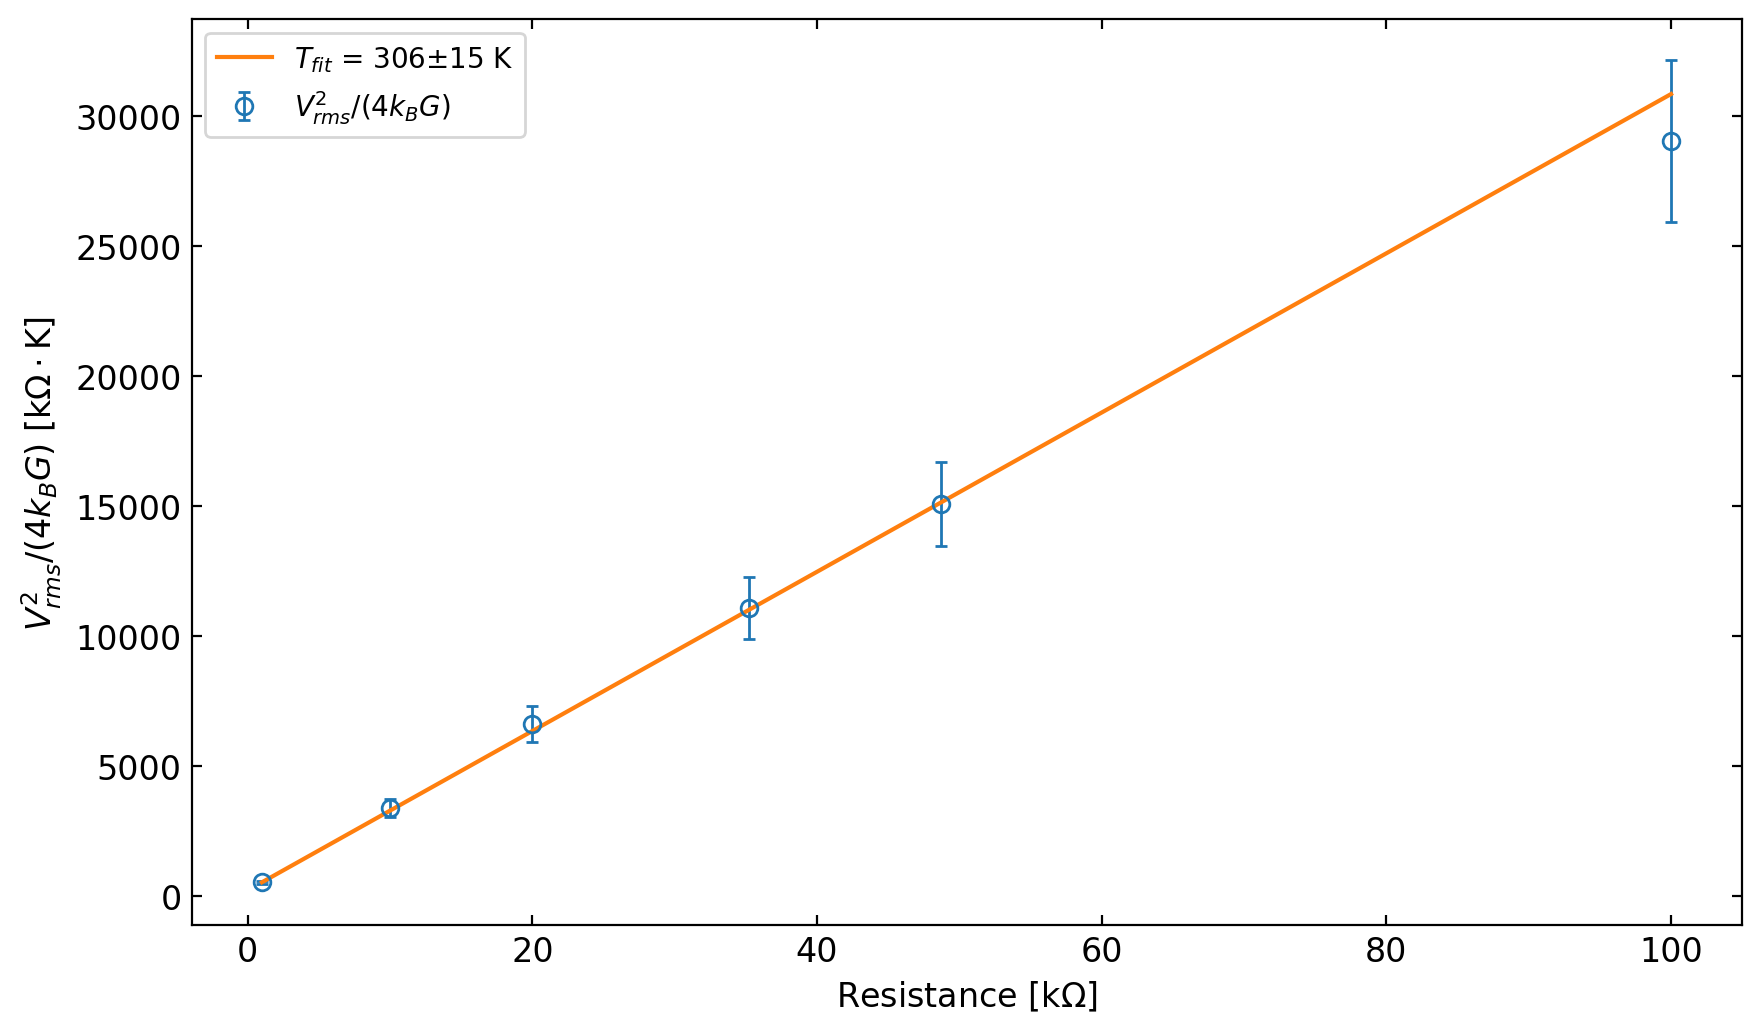
\includegraphics[width = 1\textwidth]{figures/room_temp.png}

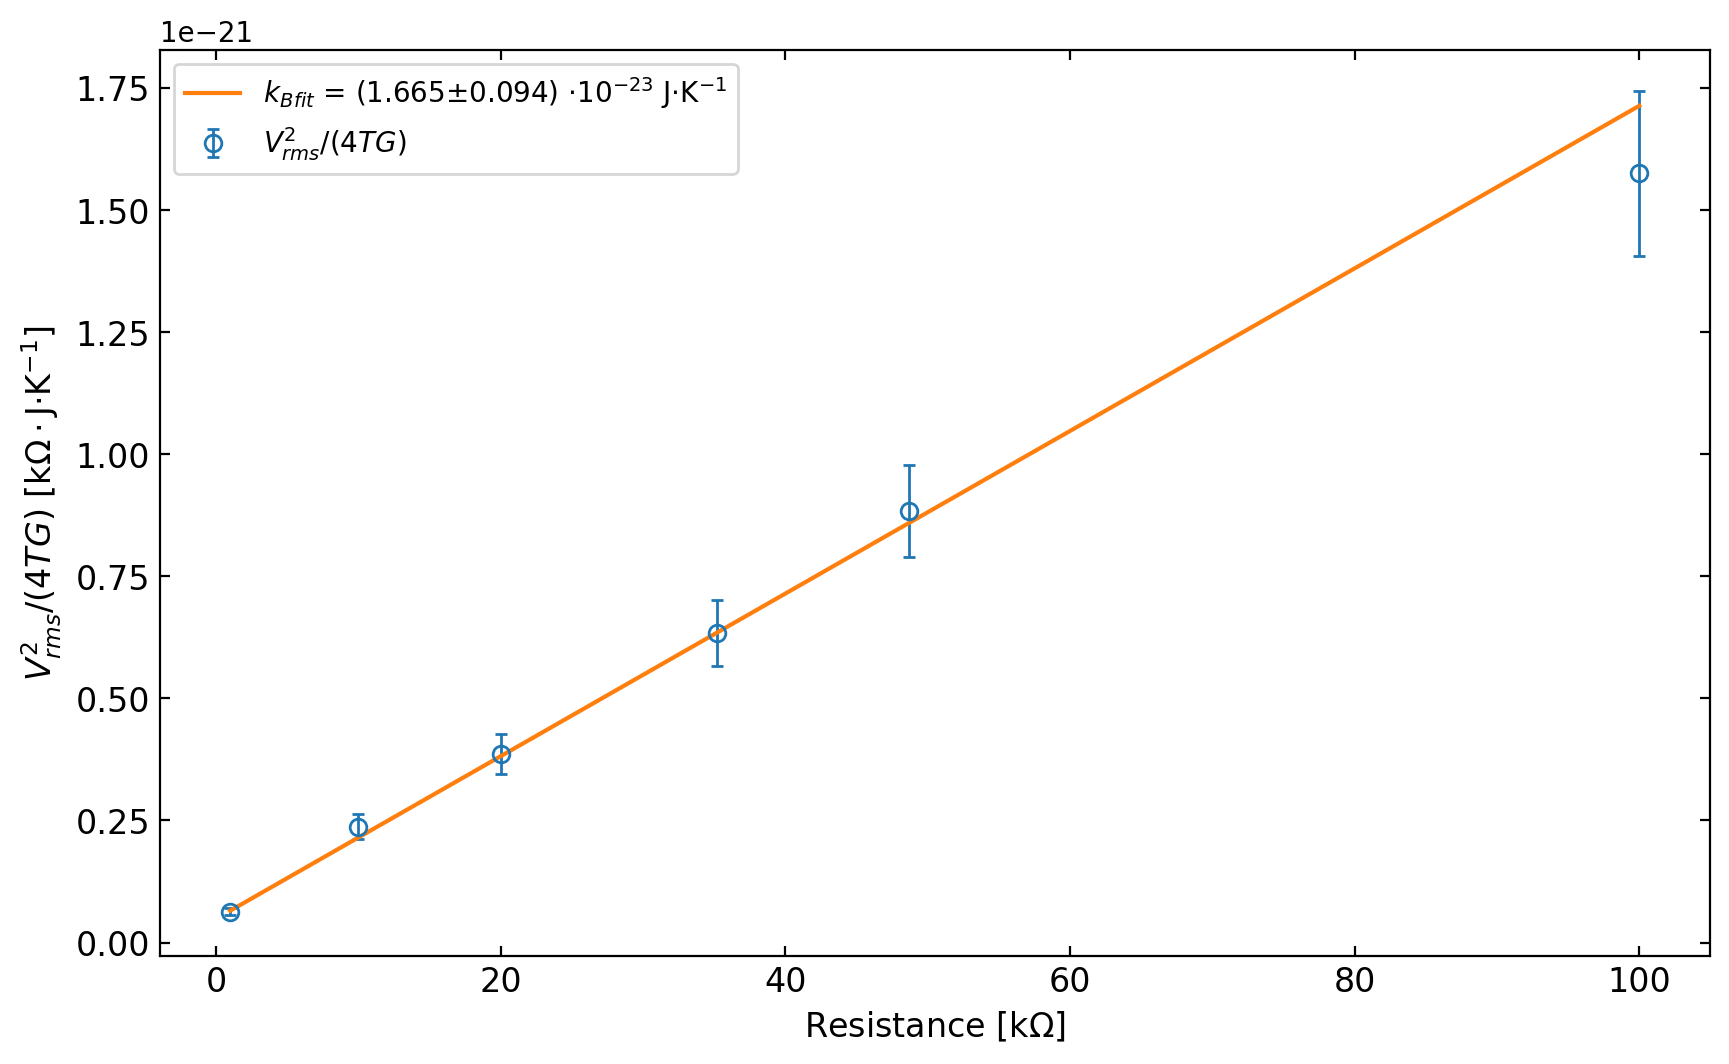
\includegraphics[width = 1\textwidth]{figures/therm_const.png}

\subsection{Error Analysis}
Error propagation follows these equations:
\begin{equation}
    \delta g = \sqrt{\left(\pdv{g}{V_{in}} \right)^2 (\delta V_{in})^2 + \left(\pdv{g}{V_{out}} \right)^2 (\delta V_{out})^2 } 
\end{equation}
\begin{equation}
    \delta G = \sqrt{\left(\pdv{G}{g} \right)^2 (\delta g)^2 + \left(\pdv{G}{R} \right)^2 (\delta R)^2  + \left(\pdv{G}{C} \right)^2 (\delta C)^2  }
\end{equation}
\begin{equation}
    \delta T = \sqrt{\left(\pdv{T}{G} \right)^2 (\delta G)^2 + \left(\pdv{T}{R} \right)^2 (\delta R)^2 + \left(\pdv{T}{V} \right)^2 (\delta V)^2} \label{eqn:temp}
\end{equation}
\begin{equation}
    \delta k_B = \sqrt{\left(\pdv{k_B}{G} \right)^2 (\delta G)^2 + \left(\pdv{k_B}{R} \right)^2 (\delta R)^2 + \left(\pdv{k_B}{V} \right)^2 (\delta V)^2}\label{eqn:therm}
\end{equation}

To measure absolute zero temperature, we used Equation~\ref{eqn:temp} to compensate for the difference between our measured results and the accepted results. However, when estimating the Boltzmann constant, the discrepancy exceeded our propagated error bars.

We deduced that the uncertainty in capacitance (C) cannot account for the upper shift in our results. Since our circuit and coaxial cables are connected in series, the total effective capacitance can only decrease, leading to an increase in gain and a decrease in the slope of the linear fit used to measure $k_B$. Furthermore, the uncertainty in resistance (R) is not significant enough to explain the deviation in our measurement.

Thus, we speculate that the calculated gain function may be inaccurate due to the presence of ambient background noise from the equipment. Notably, the background noise we measured was comparable to the un-amplified signal from the noise generator. Additionally, the measurement of white noise showed significant deviation before and after we conducted other measurements.

\begin{center}
    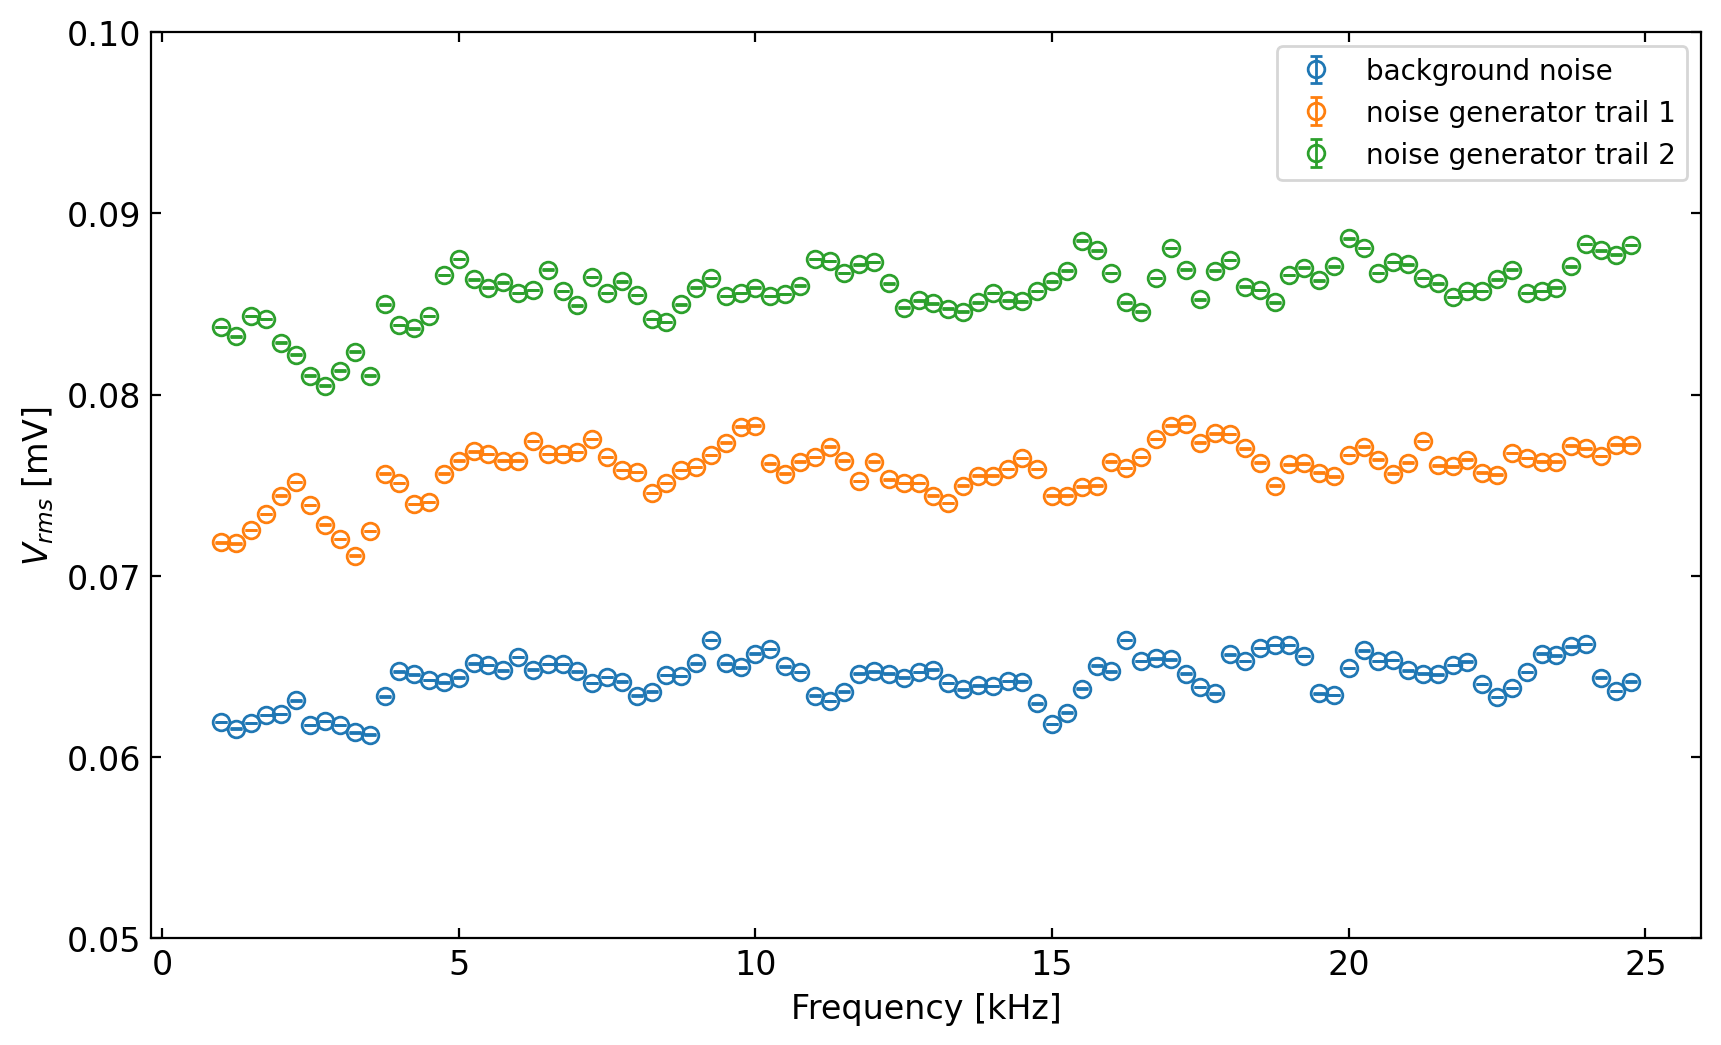
\includegraphics[width = 1\textwidth]{figures/noise_gen.png}
    \caption {Measurement of background noise of the spectral analyzer, and unprocessed signal from the random noise generator. We conducted trail 1 before measuring Johnson noise of the resistors, and trail 2 after we finished them. This plot suggests that our measurement of gain might not be stable, and the background noise will affect our system significantly.}\label{fig:noise_gen}
\end{center}





\newpage
\section{Discussion}

\quad The calculated Boltzmann constant in our experiment exhibits a significant discrepancy compared to the accepted value, with a large error. After careful consideration and experimentation, we have eliminated possible error sources from capacitance and resistance measurements. Our analysis points to the gain function $g(f)$ as the main contributor to the large error. As described above, the gain is calculated by dividing the output voltage $V_{out}$ by the input voltage $V_{in}$. We can measure $V_{out}$ with good accuracy, as its value is sufficiently large. However, $V_{in}$ is too small in comparison to the background noise, leading to inaccurate measurements and resulting in the observed large error. One possible solution to this issue is to increase the output voltage of the white noise generator, thereby decreasing the gain of the pre-amplifier. This would allow the $V_{in}$ signal to increase, making it easier to separate from the background noise.


%\hrulefill

%%%%%%%%%%%%%%%%%%%%%%%%%%%%%%%%%%%%%%%%%%%%%%%%%%%%%%%%

%\newpage
% \bibliographystyle{plain}
% \bibliography{lab_notes}

\end{document}